\documentclass{jlreq}

\usepackage{titlesec}
\usepackage{listings}
\usepackage{fancyhdr}

% url
\usepackage{url}

% \adjustbox
\usepackage{adjustbox}

% 最初の段もindent
\usepackage{indentfirst}

% tcolorboxの設定
\usepackage[most]{tcolorbox} 
\tcbuselibrary{breakable}
\tcbuselibrary{skins}
\tcbuselibrary{listingsutf8}
% タイトルのフォーマットを変更
\titleformat{\title}
  {\centering\Huge\bfseries}
  {}
  {0em} 
  {}

\titleformat{\subtitle}
  {\centering\Large\itshape}
  {}
  {0em}
  {}

\titleformat{\subsubsection}[block]
  {\normalfont\normalsize\bfseries}
  {\arabic{subsubsection}.}
  {1em}
  {}

\titleformat{\section}[block]
  {\normalfont\large\bfseries}
  {\Roman{section}.}
  {1em} 
  {}
  [\titleline{\titlerule[1pt]}]

\titleformat{\subsection}[block]
  {\normalfont\normalsize\bfseries}
  {\roman{subsection}.}
  {1em}
  {}

% listingsの設定

% 問題環境
\newtcolorbox{problem}[1][]{enhanced,
  colback=white!85!gray,
  drop fuzzy shadow,
  boxrule=0.3mm,
  arc=0mm,
  left=0pt,
  top=0pt,
  sharp corners,
  width=\textwidth,
  title=\textbf{問題},
  #1
}

\renewcommand{\lstlistingname}{コード}

\lstset{
	breaklines = true,
	language = Python,
	keywordstyle = {\bfseries \color[cmyk]{0,1,0,0}},
	commentstyle = {\itshape \color[cmyk]{1,0.4,1,0}},
	numbers = left,
	numberstyle = \tiny,
	stepnumber = 1,
	% frameとnumberの間の距離
	numbersep = 10pt,
	frame = single,
	basicstyle = \ttfamily,
	tabsize = 2,
	captionpos = t,
	backgroundcolor={\color[gray]{.90}},
	showstringspaces = false,
}

% headerの設定
\pagestyle{fancy}
\fancyhf{}

\fancyhead[RO,RE]{\rightmark}
\fancyhead[LO,LE]{\leftmark} 
\fancyfoot[C]{\thepage}

% tikzの設定
\usepackage{tikz}

\usepackage{amssymb} 

\newtcolorbox{definitionbox}[1][]{
    enhanced,
    title=#1, 
    attach boxed title to top left, 
    colback=white!95!blue,
    colbacktitle=white!10!blue!50!black,
    drop fuzzy shadow,
    boxrule=0.25mm,
}
% 定理環境
\newtcolorbox{theorembox}[1][]{
    enhanced,
    colback=white!95!green,
    colframe=green!40!black,
    coltitle=black,
    fonttitle=\bfseries,
    title=#1,
    attach boxed title to top left={yshift=-2mm, xshift=2mm},
    boxed title style={colback=green!30!white, size=small},
    drop fuzzy shadow,
    boxrule=0.5mm,
    sharp corners,
    top=4mm, bottom=4mm,
}

\usepackage[colorlinks=true, linkcolor=blue]{hyperref}

\begin{document}
\section{序論}
本書では東京大学大学院情報理工 電子情報学の受験科目の1つである情報理論について「情報理論 今井 秀樹」の問題の解説を通じて
学習していきます。問題に必要な知識を1から記述していくため、最初は冗長な記述が多いかもしれませんが、問題が進むにつれて
簡潔な記述になるように心がけます。問題のすぐ下に解答を記述しているので、解答だけを見たい場合はそれを参照してください。
\section{情報源符号化}
\begin{problem}
	\textbf{問題1.1} p.102 4.1 \\
	以下の表のような確率分布を持つ無記憶情報源を2元ハフマン符号化および4元ハフマン符号化せよ。 \\

	\begin{center}
		\begin{tabular}{|c|c|c|c|}
			\hline
			記号 & 確率 & 記号 & 確率 \\
			\hline
			$a_0$ & 0.363 & $a_4$ & 0.087 \\
			\hline
			$a_1$ & 0.174 & $a_5$ & 0.069 \\
			\hline
			$a_2$ & 0.143 & $a_6$ & 0.045 \\
			\hline
			$a_3$ & 0.098 & $a_7$ & 0.021 \\
			\hline
		\end{tabular}
	\end{center}
	\vspace{0.5cm}
	\dotfill \\
	\textbf{解答} \\
\end{problem}
情報理論の始めの問題なので詳しく解説します。まず\textbf{無記憶情報源}とは情報源が出力する\textbf{情報源記号}が他の時点の情報源記号から独立している情報源のこと
をいいます。情報源記号とは情報源から出力される記号のことです。またある情報源から出力される情報源記号の全体集合のことを\textbf{情報源アルファベット}といいます。
例えば、小文字アルファベットを出力する情報源があったとき、その情報源の情報源アルファベットは$\{a, b, c, \ldots, z\}$で、その元が情報源記号です。まとめると以下のようになります。

\begin{theorembox}[無記憶情報源]
	以下の性質を満たす情報源を無記憶情報源という。
	\begin{equation*}
		P(X_n = x_n | X_1, X_2, \ldots, X_{n-1}) = P(X_n = x_n) \quad (2 \leq n)
	\end{equation*}
\end{theorembox}

次に\textbf{ハフマン符号}について説明します。そもそも\textbf{情報源符号化}は情報源を0と1の列に変換することで、その符号化は\textbf{瞬時符号}で\textbf{平均符号長が最小}であることが望ましいです。
瞬時符号とは、ある情報源記号の符号が他の情報源記号の符号の先頭部分に一致しない符号のことです。平均符号長が最小であることは、情報源記号の符号長の平均が最小であることを意味します。
また情報源の符号化の方法は複数あるが、平均符号長を最小にする符号を\textbf{コンパクト符号}といいます。

ハフマン符号はコンパクト符号を構成する方法の1つで、以下の手順で構成されます。

\begin{theorembox}[ハフマン符号の構成]
	\begin{enumerate}
		\item 情報源アルファベットの各情報源記号に対して確率を割り当て、符号の木の葉に配置する。
		\item 確率が最小の2つの情報源記号を選び、2つの確率の和を持つ新しい富豪の木の葉とする。
		\item 1, 2を繰り返し、情報源記号が1つになるまで続ける。
	\end{enumerate}
\end{theorembox}

\textbf{符号の木}とは情報源記号の符号化を木で表現したグラフです。例えば以下の符号化の符号の木を考えます。
平均符号長は$0.6 \times 1 + 0.25 \times 2 + 0.1 \times 3 + 0.05 \times 3 = 1.55$です。

\vspace{0.5cm}

\begin{center}
\begin{tabular}{c|c|c}
	情報源記号 & 確率 & 符号 \\
	\hline
	A & 0.6 & 0 \\
	\hline 
	B & 0.25 & 10 \\
	\hline
	C & 0.1 & 110 \\
	\hline
	D & 0.05 & 111 \\
	\hline
\end{tabular}
\end{center}

\vspace{0.5cm}

この符号を符号の木で表現すると以下のようになる。符号の木では葉に情報源記号とその確率を記しておく。
エッジには0と1のいずれかを記しておく。符号の木は0と1のどちらを選んだかによって形が変わるが、平均符号長は変わらない。

\vspace{0.5cm}
\begin{center}
	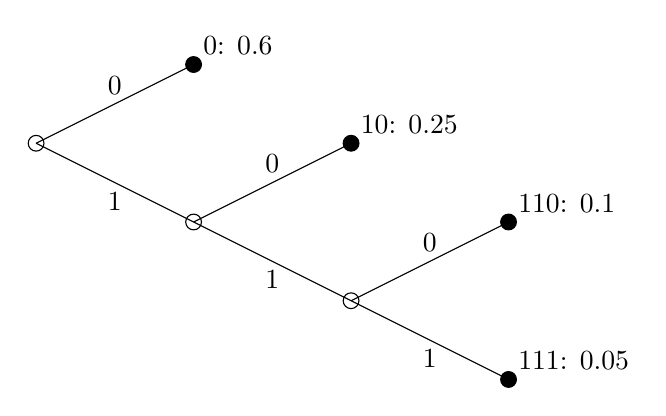
\begin{tikzpicture}
		\coordinate (A) at (0, 0);
		\draw (A) circle (0.1);
		\coordinate (B) at (2, 1);
		\draw[fill=black] (B) circle (0.1);
		\coordinate (C) at (2, -1);
		\draw (C) circle (0.1);
		\coordinate (D) at (4, 0);
		\draw[fill=black] (D) circle (0.1);
		\coordinate (E) at (4, -2);
		\draw (E) circle (0.1);
		\coordinate (F) at (6, -1);
		\draw[fill=black] (F) circle (0.1);
		\coordinate (G) at (6, -3);
		\draw[fill=black] (G) circle (0.1);

		\draw (A) -- (B) node[midway, above] {0};
		\draw (A) -- (C) node[midway, below] {1};
		\draw (C) -- (D) node[midway, above] {0};
		\draw (C) -- (E) node[midway, below] {1};
		\draw (E) -- (F) node[midway, above] {0};
		\draw (E) -- (G) node[midway, below] {1};

		% 葉の情報源記号
		\node at (B) [above right] {0: 0.6};
		\node at (D) [above right] {10: 0.25};
		\node at (F) [above right] {110: 0.1};
		\node at (G) [above right] {111: 0.05};
	\end{tikzpicture}
\end{center}

この符号化に対してハフマン符号を構成してみます。ハフマン符号の構成にならって葉に確率を割り当てます。
アルゴリズムに従って最も確率の小さい2つ(0.1と0.05)を選び、その和である0.15を持つ新しい葉を作ります。
次に0.15と0.25を選び、その和である0.4を持つ新しい葉を作ります。最後に0.4と0.6を選び、その和である1を持つ新しい葉を作ります。
最後に根から0と1を葉まで割り当てていけばハフマン符号が完成します。

ハフマン符号を表にすると以下のようになります。符号の木で扱った符号はハフマン符号だったということがわかります。

\vspace{0.5cm}

\begin{center}
	\begin{tabular}{c|c|c}
		情報源記号 & 確率 & 符号 \\
		\hline
		A & 0.6 & 0 \\
		\hline 
		B & 0.25 & 10 \\
		\hline
		C & 0.1 & 110 \\
		\hline
		D & 0.05 & 111 \\
		\hline
	\end{tabular}
\end{center}

\vspace{0.5cm}
\begin{center}
	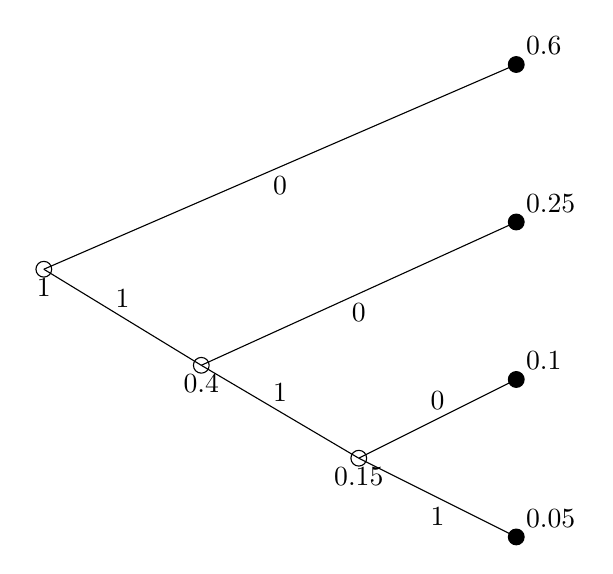
\begin{tikzpicture}
		\coordinate (A) at (4, 4);
		\draw[fill=black] (A) circle (0.1);
		\coordinate (B) at (4, 2);
		\draw[fill=black] (B) circle (0.1);
		\coordinate (C) at (4, 0);
		\draw[fill=black] (C) circle (0.1);
		\coordinate (D) at (4, -2);
		\draw[fill=black] (D) circle (0.1);

		\coordinate (E) at (2, -1);
		\draw (E) circle (0.1);
		\coordinate (F) at (0, 0.18);
		\draw (F) circle (0.1);
		\coordinate (G) at (-2, 1.4);
		\draw (G) circle (0.1);
		% 葉
		\node at (A) [above right] {0.6};
		\node at (B) [above right] {0.25};
		\node at (C) [above right] {0.1};
		\node at (D) [above right] {0.05};
		\node at (E) [below] {0.15};
		\node at (F) [below] {0.4};
		\node at (G) [below] {1};

		\draw (E) -- (C) node[midway, above] {0};
		\draw (E) -- (D) node[midway, below] {1};
		\draw (F) -- (E) node[midway, above] {1};
		\draw (F) -- (B) node[midway, below] {0};
		\draw (G) -- (F) node[midway, above] {1};
		\draw (G) -- (A) node[midway, below] {0};
	\end{tikzpicture}
\end{center}
\vspace{0.5cm}

\section{マルコフ情報源}
\begin{problem}
	\textbf{問題2.1} p.102 4.2 \\
	図のマルコフ情報源について以下の問いに答えよ。

	(1) 状態の定常分布を求めよ。\\
	(2) H(S)を求めよ。\\
	(3) $H_1(S)$を求めよ。\\
	(4) $H_2(S)$を求めよ。\\
	\dotfill \\
	\textbf{解答} \\

\end{problem}

\end{document}